\documentclass{article}
\usepackage{geometry}
 \geometry{
 a4paper,
 total={170mm,270mm},
 left=20mm,
 top=10mm,
 }
\usepackage{graphicx}
\usepackage{float}
\usepackage{enumitem}
\usepackage{caption}
\usepackage{amsmath}
\usepackage{datetime}
\usepackage{multirow}
\usepackage{listings}
\usepackage{amssymb}

\newcommand\blfootnote[1]{%
  \begingroup
  \renewcommand\thefootnote{}\footnote{#1}%
  \addtocounter{footnote}{-1}%
  \endgroup
}
\newcommand*{\addheight}[2][.5ex]{%
  \raisebox{0pt}[\dimexpr\height+(#1)\relax]{#2}%
}
\newdate{date}{18}{10}{2016}
\date{\displaydate{date}}
\title{\textbf{Network Analysis and Modelling - CSCI 5352} \\
Problem Set 4}
\author{\textbf{Santhanakrishnan Ramani}}
\begin{document}
\maketitle

\section*{Problem 1}
\blfootnote{Collaborated with Ruhi Saraf, Irene Beckman. Discussed the values and proofs for the problems after solving all by myself.}
\begin{enumerate}[label=(\alph*)]
\item
To find the expressions for $p_{in}$ and $p_{out}$, the same- and between-group parameters of the "planted partition" model's stochastic block matrix in terms of c, n, and the parameter $\epsilon = c_{in}$ - $c_{out}$.\\

Given, 
\begin{equation}
p_{in} = \dfrac{c_{in}}{n},\, p_{out} = \dfrac{c_{out}}{n}
\end{equation}
\begin{equation}
2c = c_{in} + c_{out}
\end{equation}
\begin{equation}
\epsilon = c_{in} - c_{out}
\end{equation}

Adding Eq (2) \& (3) we get,
\begin{equation}
c_{in} = \dfrac{2c + \epsilon}{2}
\end{equation}

And similarly subtracting Eq (2) \& (3) we get,
\begin{equation}
c_{out} = \dfrac{2c - \epsilon}{2}
\end{equation}

Substituting Eq (4) \& (5) in (1) we get,
$$p_{in} = \dfrac{2c + \epsilon}{2n},\, p_{out} = \dfrac{2c - \epsilon}{2n}$$

\item
The plots below shows how average epidemic size $<s>$ and length $<l>$ varies as a function of $p \in [0,1]$ for a planted partition model with n=1000, mean degree c=8, and $\epsilon=0$. The horizontal line in the length plot indicates the line $<l> = log(n)$. Since the value of $\epsilon = 0$ the probability of a vertex having connection within the same or between groups is the same, and the patterns observed in the below plots are reasonably relative to our expectations.
 
\begin{table}[H]
\centering
\begin{tabular}{|c|c|}
	\hline
	\addheight{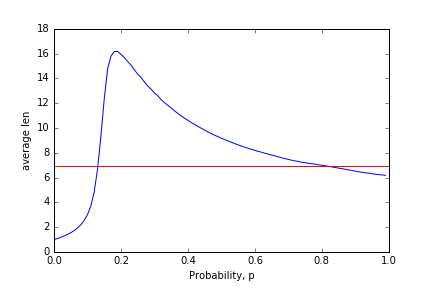
\includegraphics[width=100mm]{images/len.png}} \\
	\hline
\end{tabular}
\end{table}

We can clearly see from the length plot above that for initial values until $p \leq 0.2$ the time for which the epidemic is active increases, and once it reaches a threshold value the time for which the epidemic is active starts decreasing and tends towards the value equals the natural log of the number of nodes in the graph as $p$ increases. The former can be attributed to the fact that since the probability of infecting an edge is pretty low the epidemic is short lived, and it increases slowly reaches the highest when the probability of an edge getting infected is $\frac{1}{5}$ which is quite reasonable as in a graph with average degree equals 8 some edges gets infected and epidemic continues for a longer time. The latter can be attributed to the fact that, once the probability of an edge getting infected increases, the spread of epidemic is faster and burns out quickly,and the average length tends towards the line $<l> = log(n)$ for higher values of $p$ as the epidemic starts spreading exponentially.

\begin{table}[H]
\centering
\begin{tabular}{|c|c|}
	\hline
	\addheight{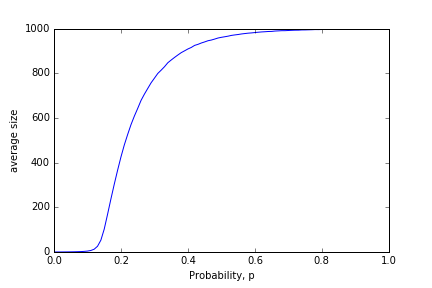
\includegraphics[width=100mm]{images/size.png}} \\
	\hline
\end{tabular}
\end{table}

Similarly, we could see the average size increases slowly initially for lower values of $p$ and after it reaches a threshold it starts increasing exponentially and the whole network gets infected for all values of $p \geq 0.75$. The reasoning for this is the same as for length, the more the probability more number of neighbouring edges gets infected and the number of nodes affected increases, and when the probability is such that 3 out of 4 edges gets infected the whole network gets infected.\\

Special values of $p$ are 0.19 when the average length reaches the maximum value, and $p$ equals 0.14 when the average size starts increasing exponentially and $p$ equals 0.76 when almost the total network starts getting infected.

\item
Plots shows some interesting behaviour of average epidemic size $<s>$ and length $<l>$ as a function of $\epsilon \in [15.5,16]$ for a planted partition model with n=200, mean degree c=8 for some interesting values of $p$.

\begin{table}[H]
\centering
\begin{tabular}{|c|c|}
	\hline
	\addheight{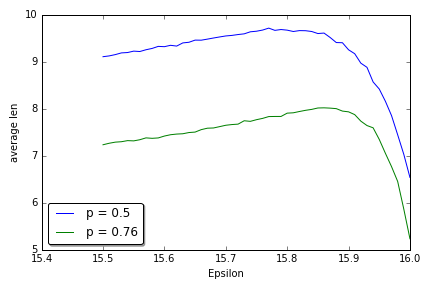
\includegraphics[width=80mm]{images/1c_len.png}} &
	\addheight{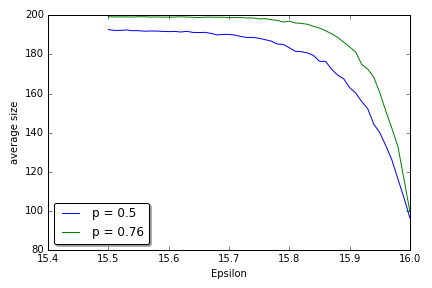
\includegraphics[width=80mm]{images/1c_size.png}} \\
	\hline
\end{tabular}
\end{table}
From the plots above we can see that there is a deviation from the intuition that we developed from 1b for these values of p, and the effect is seen in both average size and length during the same time. We see that the average size starts decreasing and it becomes almost equal to 100 the number of nodes in one group and avergae len increases a little before it goes down again when $\epsilon > 15.5$. The reason for this behaviour is because the number of edges between the two groups starts decreasing as $\epsilon$ increases and the chances of the epidemic spreading from one to another really depends on probability $p$ and the chance that one of the edges connecting the two groups gets infected.\\

The above stated behaviours can also be attributed to the community structure of the groups, if the structure is stronger the number of nodes that gets affected increases and the time taken to infect decreases within the same cluster, but at the same time the spreading of epidemic to the other cluster completely depends on any one of the connection between two groups gets infected, and when the structure is weaker the number of nodes getting infected is relatively low and the length of the epidemics too increases.\\ 

Here the transmission rule is that we flip a coin for any edge we come across and decide whether to infect it or not, since the number of chance an edge getting infected is just one, the spreading of epidemic within cluster depends on the probability an edge gets infected, but between the cluster depends on the probability as well as the number of edges between the clusters. The compromise between the probability and the value of $\epsilon$ which hints about the community structure determines the behaviour we observe in average size and len. If we relax the transmission rule a lit bit, by giving more chances then we would a completely different behaviour in average size and len.
                  	
\section*{Problem 2}
To derive an expression for the difference in modularity scores $\Delta Q = Q_2-Q_1$ and show that this difference is positive whenever $k > 2 [{c\choose2} + 1]$, the so-called resolution limit of the modularity function.\\

Given, a ring network made of k cliques each containing c vertices. We need to calculate $Q_1$ for partition $P_1$ in which there are k groups where each group contains exactly one of the k cliques and $Q_2$ for partition $P_2$ in which there are $k/2$ groups where each group contains one pair of adjacent cliques. We need to calculate $e_{uu} \,\&\, a_u$ to find the modularity given by the formula $Q = \sum_{u=1}^{k} (e_{uu} - {a_u}^2)$, where $e_{uu}$ is the number of starting and ending in the same group and $a_u$ is the number of edges ending at group u.\\

To calculate $Q_1$ since, here each clique is an group,  the number of edges in-between each group is given by $c \choose 2$, and number of edges ending at each group is 2, as it has one edge between neighbouring cliques, and the total number of edges in the ring network is $k * {c \choose 2} + k$.\\

$\therefore e_{uu} = \dfrac{2 * {c \choose 2}}{2k({c \choose 2} +1)} = \dfrac{{c \choose 2}}{k({c \choose 2} +1)}$ \& $a_u = \dfrac{2 * {c \choose 2} + 2}{2k({c \choose 2} +1)} = \dfrac{1}{k}$, \\

Substituting the values in the formula above we get,
$$Q_1 = \sum_{u=1}^{k} (\dfrac{{c \choose 2}}{k({c \choose 2} +1)} -  \dfrac{1}{k^2}) = \dfrac{(k-1){c \choose 2} - 1}{k({c \choose 2} +1)}$$

Similarly to calculate $Q_2$ since, here two neighbouring cliques form an group, the number of edges between each group is given by $2{c \choose 2} + 1$, and number of edges ending at each group is 2, as it has one edge between neighbouring cliques. 

$\therefore e_{uu} = \dfrac{2 (2 {c \choose 2} +1)}{2k({c \choose 2} +1)} = \dfrac{2{c \choose 2} +1}{k({c \choose 2} +1)}$ \& $a_u = \dfrac{2 (2 {c \choose 2} +1) + 2}{2k({c \choose 2} +1)} = \dfrac{2{c \choose 2} +2}{k({c \choose 2}+1)} = \dfrac{2}{k}$

Substituting the values in the formula above we get,
$$Q_2 = \sum_{u=1}^{k/2} (\dfrac{2*{c \choose 2} + 1}{k({c \choose 2} +1)} -  \dfrac{4}{k^2})= \dfrac{k(2*{c \choose 2} + 1) - 4({c \choose 2} +1)}{2k({c \choose 2} +1)}$$

Substituting $Q_1$ \& $Q_2$ we get,
\begin{align*}
\Delta Q &= \dfrac{k(2{c \choose 2} + 1) - 4({c \choose 2} +1)}{2k({c \choose 2} +1)} - \dfrac{(k-1){c \choose 2} - 1}{k*({c \choose 2} +1)}\\
&= \dfrac{k - 2[{c \choose 2} + 1]}{2k*({c \choose 2} +1)}
\end{align*}

So in order for $\Delta Q$ to be positive,
$$k > 2[{c \choose 2} + 1]$$
\end{enumerate}
\newpage
\section*{Code for Problem 1b}
\begin{lstlisting}[language=Python, breaklines=true]
from __future__ import division
import networkx as nx
import numpy as np
import random
from Queue import Queue

n= 1000
c = 8
l = 2
k = 500
epsilon = 0
p_in = (2*c + epsilon)/(2*n)
p_out = (2*c - epsilon)/(2*n)
sbm = [[p_in, p_out],[p_out, p_in]]

for i in range(0,100):
    print i+1
    p = i/100
    length = 0
    epidemic_size = 0
    no_of_iter = 500
    no_of_sim = 200
    for j in range(0,no_of_iter):
        G = nx.planted_partition_graph(l, k, p_in, p_out)
        for s in range(0,no_of_sim):
            infected_list = np.zeros(n)
            lst = [random.randint(0,n-1)]
            while len(lst):
                length += 1
                newList = []
                for infected_node in lst:
                    edges = G.edges(infected_node)
                    for edge in edges:
                        if(random.uniform(0, 1) <= p):
                            if(infected_list[edge[1]] != 1):
                                newList.append(edge[1])
                                infected_list[edge[1]] = 1
                lst = newList
            epidemic_size += sum(infected_list)
    file = open("/home/santa/Dropbox/NAM/Problem Set 4/Code/prob2.txt", "a")
    file.write(str(p) + "," + str(length/(no_of_iter*no_of_sim)) + "," + str(epidemic_size/(no_of_iter*no_of_sim)) + "\n")
    file.close()

import matplotlib.pyplot as plt
import pandas as pd
import numpy as np

csv_file = "/home/santa/Dropbox/NAM/Problem Set 4/Code/prob2.csv"
df = pd.read_csv(csv_file)
lst = ['len','size']
for item in lst:
    x = df['p'].tolist()
    y = df[item].tolist()
    plt.plot( x, y )
    plt.xlabel('Probability, p')
    if item == 'len':
        plt.axhline( y=np.log(1000),  color='r')
    plt.ylabel('average ' + item)
    plt.savefig("/home/santa/Dropbox/NAM/Problem Set 4/Latex/images/"+ item+".png")
    plt.clf()
\end{lstlisting}
\section*{Code for Problem 1c}
\begin{lstlisting}[language=Python, breaklines=true]
from __future__ import division
import networkx as nx
import numpy as np
import random

n= 200
c = 8
l = 2
k = 100
for i in [50,76]:
    p = i/100
    for e in range(1550,1601):
        epsilon = e/100
        p_in = (2*c + epsilon)/(2*n)
        p_out = (2*c - epsilon)/(2*n)
        sbm = [[p_in, p_out],[p_out, p_in]]
        length = 0
        epidemic_size = 0
        no_of_iter = 1000
        no_of_sim = 20
        for j in range(0,no_of_iter):
            G = nx.planted_partition_graph(l, k, p_in, p_out)
            for s in range(0,no_of_sim):
                infected_list = np.zeros(n)
                lst = [random.randint(0,n-1)]
                while len(lst):
                    length += 1
                    newList = []
                    for infected_node in lst:
                        edges = G.edges(infected_node)
                        for edge in edges:
                            if(random.uniform(0, 1) <= p):
                                if(infected_list[edge[1]] != 1):
                                    newList.append(edge[1])
                                    infected_list[edge[1]] = 1
                    lst = newList
                epidemic_size += sum(infected_list)
        file = open("/home/santa/Dropbox/NAM/Problem Set 4/Code/1c.txt", "a")
        file.write(str(p) + "," + str(epsilon) + "," + str(length/(no_of_iter*no_of_sim)) + "," + str(epidemic_size/(no_of_iter*no_of_sim)) + "\n")
        file.close()

import matplotlib.pyplot as plt
import pandas as pd
import numpy as np

csv_file = "/home/santa/Dropbox/NAM/Problem Set 4/Code/1c.csv"
df = pd.read_csv(csv_file)
lst = ['len', 'size']
for item in lst:
    x = df['p'].tolist()
    y = df[item].tolist()
    z = df['e'].tolist()
    for p in range(2):
    	plt.plot(z[p*51:(p+1)*51],y[p*51:(p+1)*51],label= 'p='+str(x[(p*51)+1]))
    plt.xlabel('Epsilon')
    plt.ylabel('average ' + item)
    plt.legend(loc='lower left', fancybox=True, shadow=True)
    plt.tight_layout()
    plt.savefig("/home/santa/Dropbox/NAM/Problem Set 4/Latex/images/1c_"+ item + ".png")
    plt.clf()
\end{lstlisting}
\end{document}
